\documentclass[tikz,border=10pt]{standalone}
\usepackage{tikz}
\usetikzlibrary{arrows.meta,positioning}

\begin{document}

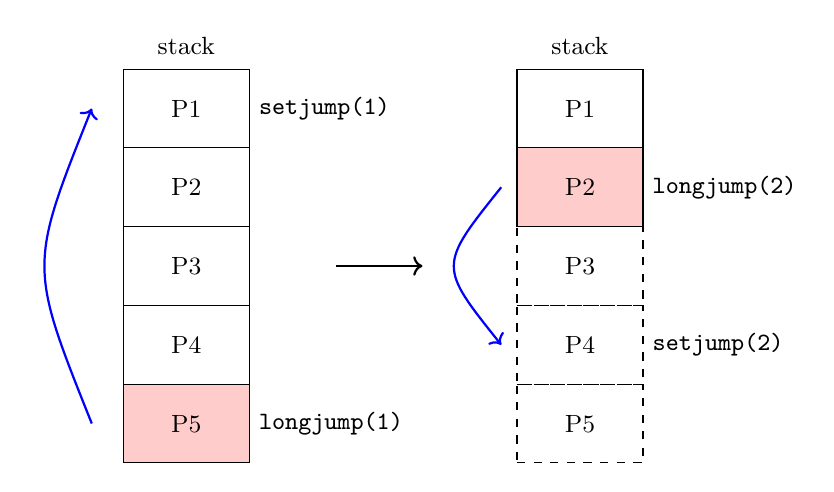
\begin{tikzpicture}[font=\small]

% ==== Left Stack ====
\node at (-2,4.8) {stack};

% Draw stack frames (left)
\foreach \name/\y in {P1/4, P2/3, P3/2, P4/1, P5/0}
    \node[draw, minimum width=1.6cm, minimum height=1cm] (L\name) at (-2,\y) {\name};

% Highlight P5
\node[draw, minimum width=1.6cm, minimum height=1cm, fill=red!20] (LP5) at (-2,0) {P5};

% setjump(1)
\draw (-1.2,4) node[right]{\texttt{setjump(1)}};

% longjump(1)
\draw (-1.2,0) node[right]{\texttt{longjump(1)}};

% Curved arrow left
\draw[->, thick, blue] (-3.2,0) .. controls (-4,2) .. (-3.2,4);


% ===== Arrow to right side =====
\draw[->, thick] (-0.1,2) -- (1.0,2);


% ==== Right Stack ====
\node at (3,4.8) {stack};

% Right stack frames (solid)
\node[draw, minimum width=1.6cm, minimum height=1cm] (RP1) at (3,4) {P1};
\node[draw, minimum width=1.6cm, minimum height=1cm, fill=red!20] (RP2) at (3,3) {P2};

% Dashed frames
\foreach \name/\y in {P3/2, P4/1, P5/0}
    \node[draw, dashed, minimum width=1.6cm, minimum height=1cm] (R\name) at (3,\y) {\name};

% longjump(2)
\draw (3.8,3) node[right]{\texttt{longjump(2)}};

% setjump(2)
\draw (3.8,1) node[right]{\texttt{setjump(2)}};

% Curved arrow right
\draw[->, thick, blue] (2,3) .. controls (1.2,2) .. (2,1);

\end{tikzpicture}

\end{document}
